% !TEX TS-program = XeLaTeX

\documentclass[usenames, xcolor=dvipsnames]{beamer}
%% \documentclass[professionalfonts, xcolor=table, handout]{beamer}
%% \usepackage{pgfpages}
%% \pgfpagesuselayout{4 on 1}[a4paper,border shrink=5mm, landscape]
%\usepackage{fontspec}
\usepackage{amsmath,amssymb}
\usepackage{pifont}% http://ctan.org/pkg/pifont
\usepackage{tikz}
\usetikzlibrary{positioning, matrix, arrows.meta, shapes.geometric, calc,
  decorations.pathmorphing, decorations.pathreplacing, fit, shapes.multipart}
\usepackage{mathabx}
\usepackage{mathtools}
\usepackage{mathpartir}
\usepackage{fancyvrb}
\usepackage{stmaryrd}
\usepackage[absolute,overlay]{textpos}
\usepackage[export]{adjustbox} % for subfigures
\usepackage[normalem]{ulem} % for strikeout
\usepackage{listings}

\lstdefinestyle{myTinyStyle}{
	%   language=Coq,
	basicstyle=\tiny,
	stepnumber=1,
	tabsize=2,
	numbers=none,
	numberstyle=\tiny,
	numbersep=5pt,
	showspaces=false,
	showstringspaces=false,
	language=C,
	morecomment=[l][{\color{OliveGreen}}]{//},
	sensitive=true,
	mathescape=true,
	escapechar=`,
	basicstyle=\tt,
	keywordstyle=\color{black},
	numbersep=5pt, boxpos=t
}

\lstset{style=myTinyStyle}

\definecolor{lightg}{RGB}{217,232,225}
\definecolor{darkg}{RGB}{6,81,42}
\definecolor{myred}{rgb}{0.0, 0.42, 0.24}
\colorlet{mypink}{myred!50!white}
\definecolor{mymaroon}{rgb}{0.86, 0.08, 0.24}

%\defaultfontfeatures{Mapping=tex-text,Scale=MatchLowercase} % HAD TO COMMENT THIS
% \setmainfont{Libertinus Serif}
% \setsansfont{Libertinus Sans}
% \setmonofont{Menlo Regular}
\usetheme{Madrid}
\useoutertheme{infolines} % Alternatively: miniframes, infolines, split
\useinnertheme{circles}

% \setbeamertemplate{enumerate item}[default]
\usecolortheme[named=myred]{structure}
% \usecolortheme{spruce}
\usefonttheme{serif}
\setbeamerfont*{frametitle}{series=\bfseries}
\setbeamercolor{alerted text}{fg=mymaroon}
\setbeamertemplate{navigation symbols}{}
\setbeamercolor{emphC}{fg=myred}
% \setbeamercolor{block title}{bg = darkg, fg=white!80}
% \setbeamercolor{block body}{bg = lightg, fg=black}
\setbeamercolor{itemize item}{fg=black}
\setbeamercolor{description item}{fg=myred}

\newcommand{\sz}{\texttt{size}}
\newcommand{\ifty}{\texttt{inf}}
\newcommand{\scon}{\mathbin{\ast}}
\usepackage{scalerel}
\renewcommand{\bigstar}{\raisebox{-0.24em}{{\scaleobj{2.5}{\scon}}}}

\newcommand{\ocon}{%
  \mathbin{\mbox{$\mathrlap{\cup}\hspace*{.15em}
      \raisebox{.01em}[0ex][0ex]{$\scon$}$\hspace*{.07em}}}}
\newcommand{\medocon}{
  \raisebox{-0.3ex}{\resizebox{0.63em}{!}{$\scon$}} \hspace{-2.4ex} \bigcup}
\newcommand{\wand}{%
 \mathrel{\mbox{$\hspace*{-0.03em}\mathord{-}\hspace*{-0.66em}
  \mathord{-}\hspace*{-0.36em}\mathord{\scon}$\hspace*{-0.005em}}}}
\newcommand{\defeq}{\mathbin{\stackrel{\Delta}{=}}}
\newcommand{\emphd}[1]{{\bfseries #1}}
\newcommand{\emphr}[2]{\alert<#1>{#2}}
\newcommand{\bracket}[1]{[#1]}
\newcommand{\hide}[1]{}
\newcommand{\braces}[1]{\color{OliveGreen}\left\{\begin{array}{l@{}} \!\!\! #1 \end{array}\right\}}
\newcommand{\s}{11}

\makeatletter\let\frametextheight\beamer@frametextheight\makeatother
\newcommand\credit[1]{%
  \begin{textblock*}{\paperwidth}(0pt,\textheight)
    \raggedleft #1\hspace{.5em}
\end{textblock*}}
\newcommand{\pguards}[1]{\llbracket #1 \rrbracket}
\newcommand{\xmark}{\ding{55}}%
\newcommand{\cmark}{\ding{51}}%
\newcommand{\m}[1]{\ensuremath{\mathit{#1}}} % math font
\newcommand{\p}[1]{\ensuremath{\mathsf{#1}}} % predicate font
\newcommand{\bi}{\Leftrightarrow} % equivalence of expressions

\AtBeginSection[]
{
  \begin{frame}
    \frametitle{Outline}
    \tableofcontents[currentsection]
  \end{frame}
}

\setbeamertemplate{section in toc}{%
  \inserttocsectionnumber.~\inserttocsection}
\setbeamercolor{subsection in toc}{bg=white,fg=structure}
\setbeamertemplate{subsection in toc}{%
  \hspace{1.2em}{\rule[0.3ex]{3pt}{3pt}}~\inserttocsubsection\par}


\title[Verifying Dijkstra, Kruskal, Prim]{Functional Correctness of Dijkstra's, Kruskal's, \\ and Prim's Algorithms in C}
\author[Mohan, Leow, Hobor]{Anshuman Mohan \qquad Leow Wei Xiang \qquad \underline{Aquinas Hobor}}
\institute[NUS]{\includegraphics[height=0.12\textwidth]{NUS_logo_full-horizontal.jpg}}
\date[]{CAV 2021 \\ July 18-24, 2021}

\begin{document}
\begin{frame}[plain]
  \titlepage
\end{frame}

\begingroup
    \AtBeginSection[]{}
\section{CertiGraph: Motivation and Overview}
\endgroup

\begin{frame}{Refresher: Dijkstra, Prim, Kruskal}

{\centering
\begin{adjustbox}{scale=0.9}
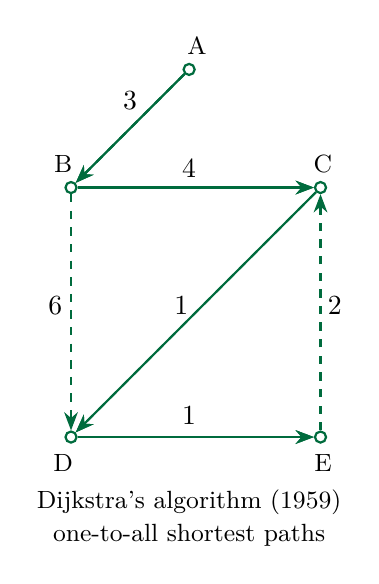
\begin{tikzpicture}
[vad/.style={rectangle, fill=black, inner sep=0pt, minimum size=4pt},
 inf/.style={circle, draw=myred, thick, inner sep=0pt, minimum size=4pt},
 inv/.style={circle, fill=myred, draw=myred, thick, inner sep=0pt, minimum size=4pt},
 ->/.style={thick, arrows={-Stealth}},
 every text node part/.style={align=center}]

% static vertices and their labels
\node at (1.6, 1.8) {\small A};
\node at (-0.1, 0.3) {\small B};
\node at (3.2, 0.3) {\small C};
\node at (-0.1, -3.5) {\small D};
\node at (3.2, -3.5) {\small E};
\node[inf] (A) at (1.5,1.5) {};
\node[inf] (B) at (0,0) {};
\node[inf] (C) [right = 3 of B] {};
\node[inf] (D) [below = 3 of B] {};
\node[inf] (E) [below = 3 of C] {};

% names
  \uncover<1,2>{\node at (1.5,-4.2) {\small Dijkstra's algorithm (1959) \\
  \small one-to-all shortest paths};}

%edge labels
\node at (.75,1.1) {3};
\node at (1.5,0.25) {4};
\node at (1.5,-2.89) {1};
\uncover<1-2>{\node at (-0.2,-1.5) {6};
			\node at (3.35,-1.5) {2};}
\uncover<1-2>{\node at (1.4,-1.5) {1};}

%edges for Dijkstra
\uncover<1,2>{
  \draw [->, dashed, myred] (A) -- (B);
  \draw [->, dashed, myred] (B) -- (C);
  \draw [->, dashed, myred] (D) -- (E);
  \draw [->, dashed, myred] (B) -- (D);
  \draw [->, dashed, myred] (E) -- (C);
  \draw [->, dashed, myred] (C) -- (D);
 }
\uncover<2>{
  \draw [->, myred] (A) -- (B);
  \draw [->, myred] (B) -- (C);
  \draw [->, myred] (D) -- (E);
  \draw [->, myred] (C) -- (D);
 }

\end{tikzpicture}
\end{adjustbox}

}% end centering
\end{frame}

\begin{frame}{Motivation: a precondition for Dijkstra}

In a graph with \texttt{size} vertices, \\
the longest possible optimal path has \texttt{size-1} links \\
\uncover<2->{so edge costs should be $\leq \lfloor\texttt{MAX/(size-1)}\rfloor$ to prevent overflow}

\bigskip \uncover<4->{
Consider a $4$-bit machine and unsigned integers \\
\texttt{MAX} = 15, \texttt{size} = 3, so every edge-cost $\le 7$.}

\bigskip

{\centering
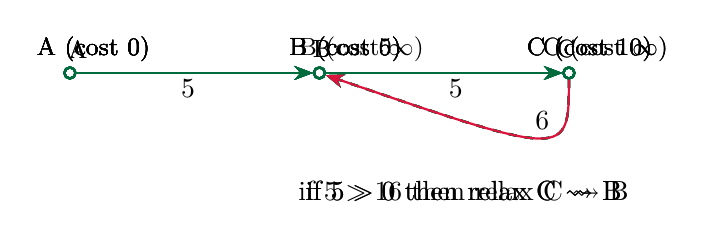
\begin{tikzpicture}
[inf/.style={circle, draw=myred, thick, inner sep=0pt, minimum size=4pt},
 ->/.style={thick, arrows={-Stealth}}]

\uncover<4->{
  \node at (1.5,-0.2) {5};
  \node at (4.9,-0.2) {5};
  \node at (6,-0.6) {6};
  }

\uncover<1-2>{
\node at (0.1, 0.3) {\small A};
\node at (3.2, 0.3) {\small B};
\node at (6.3, 0.3) {\small C};
  \node[inf] (A) at (0,0) {};
  \node[inf] (B) [right = 3 of A] {};
  \node[inf] (C) [right = 3 of B] {};
  \draw [->, dashed, myred] (A) -- (B);
  \draw [->, dashed, myred] (B) -- (C);}

\uncover<3-4>{
\node at (0.1, 0.3) {\small A};
\node at (3.2, 0.3) {\small B};
\node at (6.3, 0.3) {\small C};
  \node[inf] (A) at (0,0) {};
  \node[inf] (B) [right = 3 of A] {};
  \node[inf] (C) [right = 3 of B] {};
  \draw [->, dashed, myred] (A) -- (B);
  \draw [->, dashed, myred] (B) -- (C);
  \draw [->, dashed, myred] (C.south) .. controls ++(0, -1) .. (B);}

\uncover<5>{
\node at (0.3, 0.3) {\small A (cost 0)};
\node at (3.7, 0.3) {\small B (cost $\infty$)};
\node at (6.8, 0.3) {\small C (cost $\infty$)};
  \node[inf] (A) at (0,0) {};
  \node[inf] (B) [right = 3 of A] {};
  \node[inf] (C) [right = 3 of B] {};
  \draw [->, dashed, myred] (A) -- (B);
  \draw [->, dashed, myred] (B) -- (C);
  \draw [->, dashed, myred] (C.south) .. controls ++(0, -1) .. (B);}

\uncover<6>{
\node at (0.3, 0.3) {\small A (cost 0)};
\node at (3.5, 0.3) {\small B (cost 5)};
\node at (6.8, 0.3) {\small C (cost $\infty$)};
  \node[inf] (A) at (0,0) {};
  \node[inf] (B) [right = 3 of A] {};
  \node[inf] (C) [right = 3 of B] {};
  \draw [->, myred] (A) -- (B);
  \draw [->, dashed, myred] (B) -- (C);
  \draw [->, dashed, myred] (C.south) .. controls ++(0, -1) .. (B);
  }

\uncover<7>{
\node at (0.3, 0.3) {\small A (cost 0)};
\node at (3.5, 0.3) {\small B (cost 5)};
\node at (6.6, 0.3) {\small C (cost 10)};
  \node[inf] (A) at (0,0) {};
  \node[inf] (B) [right = 3 of A] {};
  \node[inf] (C) [right = 3 of B] {};
  \draw [->, myred] (A) -- (B);
  \draw [->, myred] (B) -- (C);
  \draw [->, dashed, myred] (C.south) .. controls ++(0, -1) .. (B);
}

\uncover<8>{
\node at (0.3, 0.3) {\small A (cost 0)};
\node at (3.5, 0.3) {\small B (cost 5)};
\node at (6.6, 0.3) {\small C (cost 10)};
\node at (5, -1.5) {if $5 > 16$ then relax C $\leadsto$ B};
  \node[inf] (A) at (0,0) {};
  \node[inf] (B) [right = 3 of A] {};
  \node[inf] (C) [right = 3 of B] {};
  \draw [->, myred] (A) -- (B);
  \draw [->, myred] (B) -- (C);
  \draw [->, dashed, myred] (C.south) .. controls ++(0, -1) .. (B);
}

\uncover<9>{
\node at (0.3, 0.3) {\small A (cost 0)};
\node at (3.5, 0.3) {\small B (cost 5)};
\node at (6.6, 0.3) {\small C (cost 10)};
\node at (5, -1.5) {if $5 > \alert{0}$ then relax C $\leadsto$ B};
  \node[inf] (A) at (0,0) {};
  \node[inf] (B) [right = 3 of A] {};
  \node[inf] (C) [right = 3 of B] {};
  \draw [->, myred] (A) -- (B);
  \draw [->, myred] (B) -- (C);
  \draw [->, dashed, myred] (C.south) .. controls ++(0, -1) .. (B);
}

\uncover<10->{
\node at (0.3, 0.3) {\small A (cost 0)};
\node at (3.5, 0.3) {\small B (cost \alert{0})};
\node at (6.6, 0.3) {\small C (cost 10)};
\node at (5, -1.5) {if $5 > 0$ then \alert{relax C $\leadsto$ B}};
  \node[inf] (A) at (0,0) {};
  \node[inf] (B) [right = 3 of A] {};
  \node[inf] (C) [right = 3 of B] {};
  \draw [->, myred] (A) -- (B);
  \draw [->, myred] (B) -- (C);
  \draw [->, mymaroon] (C.south) .. controls ++(0, -1) .. (B);
}

\end{tikzpicture}

}
\bigskip
\uncover<10->{
Must allow room for the probing edge \hide{\includegraphics[scale=.08]{nye}} \\ }
\uncover<11>{so an edge-cost is, at most, \alert{$\lfloor\texttt{MAX/size}\rfloor$}}

\end{frame}

\hide{
\begin{frame}{Motivation: A precondition for Dijkstra}

There are many ways to fix this! \pause
\\ \hspace{1em} Refactor troublesome addition as subtraction \pause
\\ \hspace{1em} Coerce to \texttt{long} \pause
\\ \hspace{1em} Work in \texttt{float}, which has $\infty^{+}$ \pause
\\ \hspace{1em} Never look back into optimized part \pause
\\ \hspace{1em} Stop earlier: when you have one vertex left in PQ, rather than zero \pause

\bigskip

Sadly, this is code directly from textbooks, and \\
intuition supports our misstep\pause{}... \\
...bugs such as this are often overlooked

\end{frame}
}

\begin{frame}{CertiGraph: problem scope}
\includegraphics[scale=0.12]{compcert_logo}
\hspace{2em} \includegraphics[scale=0.09]{vst_logo}
\hspace{2em} \includegraphics[scale=0.2]{paper_screen}

\bigskip
CompCert + VST + \underline{CertiGraph}

\bigskip

\pause

Verify executable graph-manipulating code with rich specifications
%\\\hspace{1em}expressed with mathematical graphs

\end{frame}

\begin{frame}{Major contributions}
\uncover<1->{
Math, spatial support for adjacency matrices, edge lists \\}
\uncover<2->{
Added support for undirected graphs \\ }
\bigskip
\uncover<3->{
Dijkstra: nontrivial overflow \\ }
\uncover<4->{
Prim: nontrivial improvement in spec \\ }
\uncover<5->{
Kruskal: library handles directed $+$ undirected \\ }
\uncover<6->{
Binary heap: \texttt{decrease-key} and \texttt{heapify}, avoids overflow \\ }
\bigskip
\uncover<7->{
Development is modular and general% \\
%High effort---largely because we work with C---but good reuse
}
\bigskip
\uncover<8->{
\flushright
Thanks! \hspace{2em}}
\end{frame}

\end{document}
